% === [ Literature Review ] ====================================================

% <howto>
% * Critical review of relevant literature
%    - Not just what others have said, but also critique and reflect

% <howto> Doing a literature review
% * Define the problem
% * Literature search
% * Literature review
%    - Read and evaluate the literature
%    - Critically analyse what you have found
% * More than one iteration (continue throughout the project)

% <howto> suggested review approaches
% * Thematic
%    - explain about area of study: general review of area, concentrating on
%      academic literature
% * More focused
%    - e.g. some recent developments in the field
% * Chronological
%    - how the topic has evolved (but beware palaeontology)
% * Alternative theories and methods and explanation why they are relevant
% * SHORT overview of relevant tools

% <howto> literature search
% * Start broad, then focus
% * Redefine/refine search
%    - Continuous cycle: identify different thinking in the area

% <howto> marking notes
% * Uses credible, current material
% * Demonstrates understanding of complex subject and viewed in wider context
% * Shows originality and confidence in criticising assumptions
% * Well-justified critique of literature
% * Identifies flaws, gaps or inconsistencies in extant knowledge

% <howto>
% * What is the problem, or research question that my literature review helps to
%   define?
% * What is the scope of my literature review?
% * Has my search been wide enough to ensure I've found all the relevant
%   material and narrow enough to exclude irrelevant material?
% * Have I critically analysed the literature I use? Do I follow through a set
%   of concepts and questions, comparing items to each other in the ways they
%   deal with them? Instead of just listing and summarizing items, do I assess
%   them, discussing strengths and weaknesses?
% * IMPORTANT: Have I cited and discussed studies contrary to my perspective?

% <howto>
% * Write brief notes on each source (your own words, not their abstract):
%    - Key ideas (seminal sources, recognized theories)
%    - Novel ideas (proposed or demonstrated)
%    - Actual data (as distinct from mere argument)
%    - Outliers (contradict what everyone else says)
%    - Your critical evaluation: Is it convincing? Why? What are its
%      limitations? Is it current or out-of-date? What does it fail to address?

% <howto> common mistakes in writing a literature review
% * Writing your own opinion on a particular subject
% * Writing a list of summaries of sources , one after another, without
%   reviewing it
% * Writing an essay on everything you know about a particular subject

% <howto> What is a literature review?
% * A critical look at the published work relevant to your project
% * Gives the reader understanding of the problem area and the rationale for
%   what you are doing
% * What has already been done in your area
% * Sets the context for your project
% * Justifies your project

% <howto>
% * Main themes and key authors

% <howto>
% * a literature review is NOT an essay.
%    - NOT a detailed write up of a particular source.
%    - NOT just a summary of articles, texts or journals.
%    - NOT an opinionated or argumentative essay.
%
% --- [ essay ] ---
% * Use material to prove an argument or point of view, demonstrate
%   understanding.
% * Use relevant material.
% * Mentions authors/researchers only for reference.
%
% --- [ literature review ] ---
%
% * Critical analysis of material discovered about a subject.
% * Examine what has already been discovered.
% * Find patterns, gaps, conflicts.
% * Identify key researchers.
%
% * critical appraisal: the ability to apply principles of analysis to identify
%   unbiased and valid work.

% <howto>
% * What to notice when reading
%     - What is the line of reasoning?
%     - Is evidence presented? Does it stand up? (valid criteria)
%     - What do I think about it? Do I agree? Have I found supporting /
%       contradicting material?
%     - Are there assumptions / hidden agendas?
%     - What are the writer's conclusions? Does the evidence support them?
%     - Do not just select the parts of the literature that agree with what you
%       think

% <howto>
% * which authors support which views?
% * are there inconsistencies, gaps...?

\section{Literature Review}
\label{sec:literature_review}

% TODO: <note> remove?
% This section introduces a shared vocabulary, and discussess key concepts and ideas.

foo

% TODO: <note> Problems.
%
% * self-modifying code
% * idioms
%    - mul/div by powers of 2; left-shift/right-shift
%    - long word addition
%       add ecx, [ebp-8]
%       add edx, [ebp-4]
% * Architecture-dependent Restrictions
%    Cannot be determined by step-by-step debugging; as the prefetch pipeline
%    would behave differently.
%       mov ax, 0x9090
%       mov [jmpDef], ax
%    jmpDef:
%       jmp codeExecuted
%    codeNotExecuted:
%       foo
%    codeExecuted:
%       bar
% * Subroutines included by the compiler and linker
%    Bloat.


% --- [ The Anatomy of an Executable ] -----------------------------------------

\subsection{The Anatomy of an Executable}
\label{sec:executable_anatomy}

The representation of executables, shared libraries and relocatable object code is standardized by a variety of file formats which provides encapsulation of assembly instructions and data. Two such formats are the Portable Executable (PE) file format and the Executable and Linkable Format (ELF), which are used by Windows and Linux respectively. Both of these formats partition executable code and data into sections and assign appropriate access permissions to each section, as summarised by table \ref{tbl:elf_sections}. In general, no single section has both write and execute permissions as this could compromise the security of the system.

\begin{table}[htbp]
	\begin{center}
		\begin{tabular}{|l|l|l|}
			\hline
			Section name & Usage description & Access permissions \\
			\hline
			\texttt{.text} & Assembly instructions & \texttt{r-x} \\
			\texttt{.rodata} & Read-only data & \texttt{r--} \\
			\texttt{.data} & Data & \texttt{rw-} \\
			\texttt{.bss} & Uninitialized data & \texttt{rw-} \\
			\hline
		\end{tabular}
	\end{center}
	\caption{A summary of the most commonly used sections in ELF files. The \texttt{.text} section contains executable code while the \texttt{.rodata}, \texttt{.data} and \texttt{.bss} sections contains data in various forms.}
	\label{tbl:elf_sections}
\end{table}

To gain a better understanding of the anatomy of executables the remainder of this section describes the structure of ELF files and presents the dissection of a simple \textit{``hello world''} ELF executable, largely inspired by Eric Youngdale's article on \textit{The ELF Object File Format by Dissection} \cite{elf_dissection}. Although the ELF and PE file formats differ with regards to specific details, the general principles are applicable to both formats.

In general, ELF files consist of a file header, zero or more program headers, zero or more section headers and data referred to by the program or section headers, as depicted in figure \ref{fig:elf_file_structure}.

\begin{figure}[htbp]
	\begin{center}
		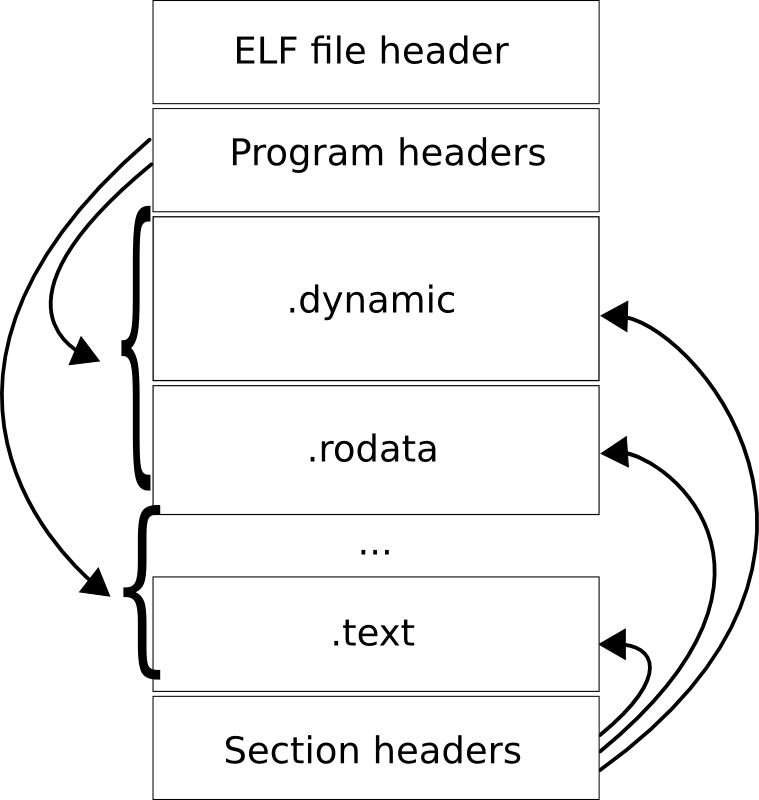
\includegraphics[width=0.5\textwidth]{inc/elf_file_structure.png}
		\caption{The basic structure of an ELF file. \textit{Image license:} CC BY-SA \cite{elf_structure_orig}}
		\label{fig:elf_file_structure}
	\end{center}
\end{figure}

All ELF files starts with the four byte identifier \texttt{0x7F}, \texttt{'E'}, \texttt{'L'}, \texttt{'F'} which marks the beginning of the ELF file header. The ELF file header contains general information about a binary, such as its object file type (executable, relocatable or shared object), its assembly architecture (x86-64, ARM, …), the virtual address of its entry point which indicates the starting point of program execution, and the file offsets to the program and section headers.

Each program and section header describes a continuous segment or section of memory respectively. In general, segments are used by the linker to load executables into memory with correct access permissions, while sections are used by the compiler to categorize data and instructions. Therefore, the program headers are optional for relocatable and shared objects, while the section headers are optional for executables.

\begin{figure}[htbp]
	\begin{center}
		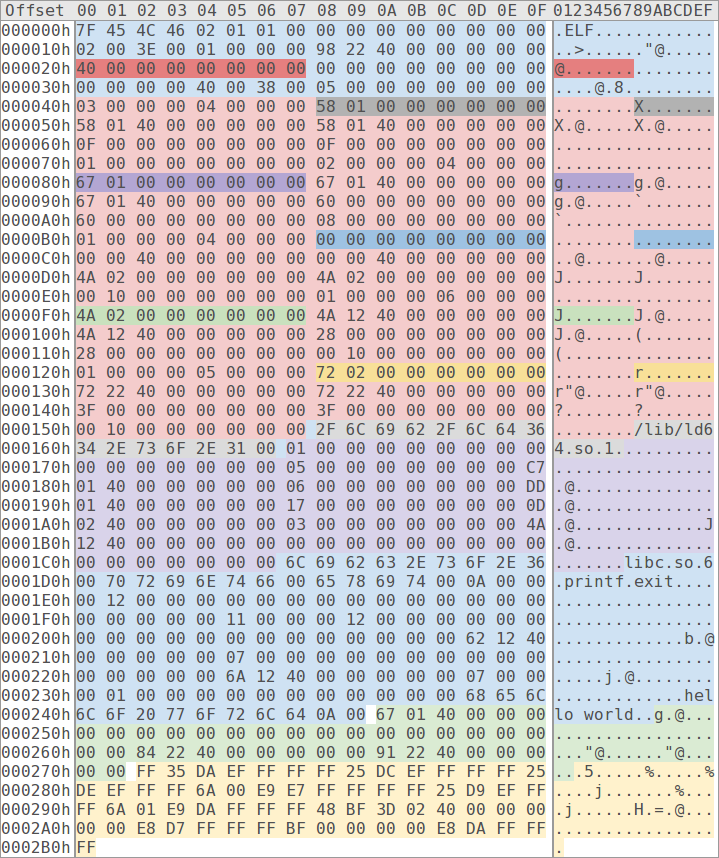
\includegraphics[width=\textwidth]{inc/elf_dissection.png}
		\caption{The entire contents of a simple \textit{``hello world''} ELF executable with colour-coded file offsets, sections, segments and program headers. Each file offset is 8 bytes in width and coloured using a darker shade of its corresponding segment, section or program header.}
		\label{fig:elf_dissection}
	\end{center}
\end{figure}

To further investigate the structure of ELF files a simple 64-bit \textit{``hello world''} executable has been dissected and its content colour-coded. Each file offset of the executable consists of 8 bytes and is denoted in figure \ref{fig:elf_dissection} with a darker shade of the colour used by its corresponding target segment, section or program header. Starting at the middle of the ELF file header, at offset \texttt{0x20}, is the file offset (red) to the program table (bright red). The program table contains five program headers which specify the size and file offsets of two sections and three segments, namely the \texttt{.interp} (gray) and the \texttt{.dynamic} (purple) sections, and a \textit{read-only} (blue), a \textit{read-write} (green) and a \textit{read-execute} (yellow) segment.

Several sections are contained within the three segments. The \textit{read-only} segment contains the following sections:

\begin{itemize}
	\item \texttt{.interp}: the interpreter, i.e. the linker
	\item \texttt{.dynamic}: array of dynamic entities
	\item \texttt{.dynstr}: dynamic string table
	\item \texttt{.dynsym}: dynamic symbol table
	\item \texttt{.rela.plt}: relocation entities of the PLT
	\item \texttt{.rodata}: read-only data section
\end{itemize}

The \textit{read-write} segment contains the following section:

\begin{itemize}
	\item \texttt{.got.plt}: Global Offset Table (GOT) of the PLT (henceforth referred to as the GOT as this executable only contains one such table)
\end{itemize}

And the \textit{read-execute} segment contains the following sections:

\begin{itemize}
	\item \texttt{.plt}: Procedure Linkage Table (PLT)
	\item \texttt{.text}: executable code section
\end{itemize}

Seven of the nine sections contained within the executable are directly related to dynamic linking. The \texttt{.interp} section specifies the linker (in this case \textit{``/lib/ld64.so.1''}) and the \texttt{.dynamic} section an array of dynamic entities containing offsets and virtual addresses to relevant dynamic linking information. In this case the dynamic array specifies that \textit{``libc.so.6''} is a required library, and contains the virtual addresses to the \texttt{.dynstr}, \texttt{.dynsym}, \texttt{.rela.plt} and \texttt{.got.plt} sections. As noted, even a simple \textit{``hello world''} executable requires a large number of sections related to dynamic linking. Further analysis will reveal their relation to each other and describe their usage.

The dynamic string table contains the names of libraries (e.g. \textit{``libc.so.6''}) and identifiers (e.g. \textit{``printf''}) which are required for dynamic linking. Other sections refer to these strings using offsets into \texttt{.dynstr}. The dynamic symbol table declares an array of dynamic symbol entities, each specifying the name (e.g. offset to \textit{``printf''} in \texttt{.dynstr}) and binding information (local or global) of a dynamic symbol. Both the \texttt{.plt} and the \texttt{.rela.plt} sections refers to these dynamic symbols using array indicies. The \texttt{.rela.plt} section specifies the relocation entities of the PLT; more specifically this section informs the linker of the virtual address to the \texttt{.printf} and \texttt{.exit} entities in the GOT.

To reflect on how dynamic linking is accomplished on a Linux system lets review the assembly instructions of the executable \texttt{.text} and \texttt{.plt} sections as outlined in listing \ref{lst:elf_text,lst:elf_plt} respectively.

\lstinputlisting[language=nasm, style=nasm, caption={The assembly instructions of the \texttt{.text} section. \label{lst:elf_text}}]{inc/elf_text.asm}

\lstinputlisting[language=nasm, style=nasm, caption={The assembly instructions of the \texttt{.plt} section. \label{lst:elf_plt}}]{inc/elf_plt.asm}

As visualized in listing \ref{lst:elf_text} the first call instruction of the \texttt{.text} section targets the \texttt{.printf} label of the \texttt{.plt} section instead of the actual address of the \textit{printf} function in the \textit{libc} library. The Procedure Linkage Table (PLT) provides a level of indirection between call instructions and actual function (procedure) addresses, and contains one entity per external function as outlined in listing \ref{lst:elf_plt}. The \texttt{.printf} entity of the PLT contains a jump instruction which targets the address stored in the \texttt{.printf} entity of the GOT. Initially this address points to the next instruction, i.e. the instruction denoted by the \texttt{.resolve\_printf} label in the PLT. On the first invokation of \textit{printf} the linker replaces this address with the actual address of the \textit{printf} function in the \textit{libc} library, and any subsequent invokation of \textit{printf} will target the resolved function address directly.

This method of external function resolution is called lazy dynamic linking as it postpones the work and only resolves a function once it is actually invoked at runtime. The lazy approach to dynamic linking may improve performance by limiting the number of symbols that require resolution. At the same time the eager approach may benefit latency sensitive applications which cannot afford the cost of dynamic linking at runtime.

A closer look at the instructions denoted by the \texttt{.resolve\_printf} label in listing \ref{lst:elf_plt} reveals how the linker knows which function to resolve. Essentially the \textit{dl\_runtime\_resolve} function is invoked with two arguments, namely the dynamic symbol index of the \textit{printf} function and a pointer to a linked list of nodes, each refering to the \texttt{.dynamic} section of a shared object. Upon termination the linked list of our \textit{``hello world''} process contains a total of four nodes, one for the executable itself and three for its dynamically loaded libraries, namely \textit{linux-vdso.so.1}, \textit{libc.so.6} and \textit{ld64.so.1}.

To summarise, the execution of a dynamically linked executable can roughly be described as follows. Upon execution the kernel parses the program headers of the ELF file, maps each segment to one or more pages in memory with appropriate access permissions, and transfers the control of execution to the linker (\textit{``/lib/ld64.so.1''}) which was loaded in a similar fashion. The linker is responsible for initiating the addresses of the \textit{dl\_runtime\_resolve} function and the aforementioned linked list, both of which are stored in the GOT of the executable. After this setup is complete the linker transfers control to the entry point of the executable, as specified by the ELF file header (in this case the \texttt{.start} label of the \texttt{.text} section). At this point the assembly instructions of the application are executed until termination and external functions are lazily resolved at runtime by the linker through invocations to the \textit{dl\_runtime\_resolve} function.

% --- [ Decompilation Phases ] -------------------------------------------------

\subsection{Decompilation Phases}
\label{sec:decompilation_phases}

A core principle utilized in decompilers is the separation of concern through the use of abstractions, and extensive work involves translating into and breaking out of various abstraction layers. In general, a decompiler is composed of distinct phases which parses, analyses or transforms the input. These phases are conceptually grouped into three modules to separate concerns regarding source machine language and target programming language. Firstly, the front-end module parses executable files and translates their platform dependent assembly into a platform independent intermediate representation (IR). Secondly, the middle-end module performs a set of decompilation passes to lift the IR, from a low-level to a high-level representation, by reconstructing high-level control structures and expressions. Lastly, the back-end module translates the high-level IR to a specific target programming language \cite{rev_comp}. Figure \ref{fig:modules_overview} gives an overview of the decompilation modules and visualizes their relationship.

\begin{figure}[htbp]
	\begin{center}
		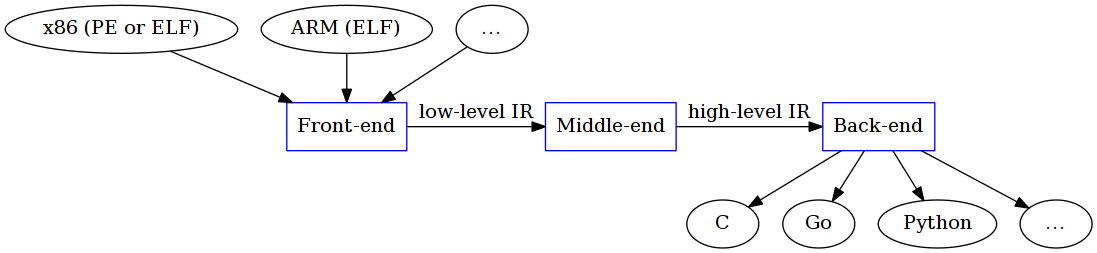
\includegraphics[width=\textwidth]{inc/modules_overview.png}
		\caption{Firstly, the front-end module accepts several executable file formats (PE, ELF, …) as input and translates their platform dependent assembly (x86, ARM, …) to a low-level IR. Secondly, the middle-end module then lifts the low-level IR to a high-level IR through a set of decompilation passes. Lastly, the backend-module translates the high-level IR into one of several target programming languages (C, Go, Python, …).}
		\label{fig:modules_overview}
	\end{center}
\end{figure}

The remainder of this section describes the distinct decompilation phases, most of which have been outlined by Cristina Cifuentes in her influential paper \textit{``Reverse Compilation Techniques''} \cite{rev_comp}.

% ~~~ [ Binary Analysis ] ~~~~~~~~~~~~~~~~~~~~~~~~~~~~~~~~~~~~~~~~~~~~~~~~~~~~~~

\subsubsection{Binary Analysis}
\label{sec:binary_analysis}

As demonstrated in section \ref{sec:executable_anatomy} parsing even a simple \textit{``hello world''} executable requires extensive knowledge of its binary file format (in this case ELF). The binary analysis phase is responsible for parsing input files of various binary file formats, such as PE and ELF, and present their content in a uniform manner which preserves the relations between file contents, virtual addresses and access permissions. Later stages of the decompilation pipeline builds upon this abstraction to access the file contents of each segment or section without worrying about the underlying file format. Information about external symbols, metadata and the computer architecture of the assembly may also be provided by this abstraction.

% ~~~ [ Disassembly ] ~~~~~~~~~~~~~~~~~~~~~~~~~~~~~~~~~~~~~~~~~~~~~~~~~~~~~~~~~~

\subsubsection{Disassembly}

The disassembly phase (referred to as the syntactic analysis phase in C. Cifuentes paper) is responsible for decoding the raw machine instructions of the executable segments into assembly. At first sight it may seem trivial to implement a disassembler; simply use a lookup table which translates a sequence of bytes to their corresponding assembly instructions.

foo

% TODO: Introduce the various approaches and highlight their individual
% strengths and weaknesses.
%
% NAIVE APPROACH: linear descent disassemblers.
% PROBLEM: Highlight problems with linear descent disassemblers.
%    - rodata (e.g. "hello world") and jump tables in code.
%
% SOLUTION: recursive descent disassemblers.
% PROBLEM: Highlight problems with recursive descent disassemblers.
%    - Distinguish between code and data (e.g. find entry points of functions).
%      Not add functions are directly referred to (e.g. callback functions which
%      are commonly used by GUI applications).
%    - Easy to fool.
%       xor eax, eax
%       cmp eax, 0
%       jz foo+1 ; Cannot disassembly both foo and foo+1.
% foo:
%       add eax, 3
%
% SOLUTION: symbolic execution engines.
% PROBLEM: security, performance, ...?

% ~~~ [ Semantic Analysis ] ~~~~~~~~~~~~~~~~~~~~~~~~~~~~~~~~~~~~~~~~~~~~~~~~~~~~

\subsubsection{Semantic Analysis}

foo

% TODO: Ideoms
%    - 64-bit binops
%    - xor eax, eax ; eax = 0

% ~~~ [ Intermediate Code Generation ] ~~~~~~~~~~~~~~~~~~~~~~~~~~~~~~~~~~~~~~~~~

\subsubsection{Intermediate Code Generation}

% TODO: <note> remove?
% "Most compilers translate the source program first to some form of intermediate representation and convert from there into machine code. The intermediate representation is a machine- and language-independent version of the original source code. Although converting the code twice introduces another step, use of an intermediate representation provides advantages in increased abstraction, cleaner separation between the front and back ends, and adds possibilities for re-targeting/cross-compilation. Intermediate representations also lend themselves to supporting advanced compiler optimizations and most optimization is done on this form of the code."

foo

% ~~~ [ Control Flow Graph Generation ] ~~~~~~~~~~~~~~~~~~~~~~~~~~~~~~~~~~~~~~~~

\subsubsection{Control Flow Graph Generation}

foo

% ~~~ [ Data Flow Analysis ] ~~~~~~~~~~~~~~~~~~~~~~~~~~~~~~~~~~~~~~~~~~~~~~~~~~~

\subsubsection{Data Flow Analysis}

foo

\cite{type_decomp}

% ~~~ [ Control Flow Analysis ] ~~~~~~~~~~~~~~~~~~~~~~~~~~~~~~~~~~~~~~~~~~~~~~~~

\subsubsection{Control Flow Analysis}

Control-Flow Graph (CFG)

foo

% TODO: Add notes about irriducible graphs; may be solved using node splitting.
% * functional (semantics?) vs. forensic equivalence.

% ~~~ [ Type Analysis ] ~~~~~~~~~~~~~~~~~~~~~~~~~~~~~~~~~~~~~~~~~~~~~~~~~~~~~~~~

\subsubsection{Type Analysis}

% TODO: Reformulate and check Mycroft reference.

The purpose of the type analysis stage is to infer the types of variables, parameters and functions. The main method for obtaining this information is through type constraint equations as pioneered by A. Mycroft
% xxx pioneered the use of type-inference through the use of type constraints equations.

type-inference

The main purpose of the type analysis stage is to infer the types of variables and parameters.




In contrast to A. Mycroft et al. \cite{type_decomp}, I. Guilfanov argues that the type analysis stage should be deferred to as late as possible. Only then may one resonably solve the type equations \cite{hexrays}.

foo

% ~~~ [ Code Generation ] ~~~~~~~~~~~~~~~~~~~~~~~~~~~~~~~~~~~~~~~~~~~~~~~~~~~~~~

\subsubsection{Code Generation}

foo

% --- [ Evaluation of Intermediate Representations ] ---------------------------

\subsection{Evaluation of Intermediate Representations}

% TODO: Very interesting read about the evaluation of IRs specifically for reverse engineering: An Intermediate Representation for Integrating Reverse Engineering Analyses.

% TODO: Check http://indefinitestudies.org/2009/04/03/a-quick-survey-on-intermediate-representations-for-program-analysis/

% TODO: Consider if this text belongs here, if it should be adapted to fit or if it should be removed entirely.

\textbf{NOTE}: \textit{The following paragraph has been moved here from another section and will therefore feel out of place. The intention is to reformulate it.}

In recent years other research groups have started to develop decompilers and reverse engineering components which rely on LLVM IR \cite{decomp_llvm,retargetable_decomp,mcsema}. An IR may exist which is more suitable in theory, but in practise the collaboration and reuse of others efforts made possible by the vibrant LLVM community is a strong merit in and of itself. The project may therefore be successful without even identifying an optimal IR for decompilation (objective \ref{itm:obj_review_suitable_ir}).

% ~~~ [ REIL ] ~~~~~~~~~~~~~~~~~~~~~~~~~~~~~~~~~~~~~~~~~~~~~~~~~~~~~~~~~~~~~~~~~

\subsubsection{REIL}

The Reverse Engineering Intermediate Language (REIL) is a very simple and platform independent assembly language. REIL's instruction set contains only 17 different instructions, each with exactly three (possibly empty) operands. The first two operands are always used for input and the third for output (except for the conditional jump instruction which uses the third operand as the jump target). Furthermore, each instruction has at most one effect on the global state and never any side-effects (such as setting flags) \cite{reil,reil_spec}.

% TODO: Operands have a type, a value and a size.

Thanks to the simplicity of REIL a full definition of its instruction set has been provided in appendix \ref{app:reil_instructions}, which includes examples of each instruction and defines their syntax and semantics (in pseudo C-code).

% TODO: Incorporate notes from "REIL - notes.txt"

The language was originally designed to assist static code analysis and translators from native assembly (x86, PowerPC-32 and ARM-32) to REIL are commercially available. However, the project home page has not been updated since Google acquired zynamics in 2011. Since then approximately 10 papers have been published which references REIL and the adaptation of the language within the open source community seems limited. As of 2015-01-04 only three implementations existed on GitHub (two in Python \cite{barf,pyreil} and one in C \cite{bit}), and the most popular had less than 25 watchers, 80 stars and 15 forks.

% ~~~ [ LLVM IR ] ~~~~~~~~~~~~~~~~~~~~~~~~~~~~~~~~~~~~~~~~~~~~~~~~~~~~~~~~~~~~~~

\subsubsection{LLVM IR}

% TODO: <note> remove?
% * Hierarchical structured
%    - Module
%       ~ Global Variables
%       ~ Composite Types (“structs”)
%       ~ Function Declarations
%       ~ Function Definitions
%    - Function Definition
%       ~ Basic Blocks
%          - Instructions

% TODO: <note> reformulate!
% LLVM IR is actually defined in three isomorphic forms: the textual format above, an in-memory data structure inspected and modified by optimizations themselves, and an efficient and dense on-disk binary "bitcode" format.


foo
